\documentclass[a4paper,11pt]{article}

\renewcommand\bottomfraction{0.9} % default value: 0.3
\renewcommand\textfraction{0.1}   % default value: 0.2

\usepackage{caption}
\usepackage{array}
\usepackage{fullpage, setspace, url}
\usepackage{colortbl}
\usepackage{amsmath}
\usepackage{indentfirst}
%\usepackage{algorithm,algorithmic}
%\definecolor{G6}{rgb}{0.7,0.7,0.7}
%\newcommand{\fc}{\cellcolor{G6}}
\usepackage{subfigure}
\usepackage{multirow}
\usepackage[table]{xcolor}
\usepackage{graphicx} 
\usepackage{bmpsize}
\usepackage{pgfgantt}

% pacotes malucões
\usepackage{graphicx}
\usepackage{amsfonts}
\usepackage{amssymb}
\usepackage{amstext}
\usepackage{hyperref}
\usepackage{ragged2e}
\usepackage{color}
\usepackage{enumerate}
\usepackage{float}
% fonte
\usepackage{helvet}
% coisas de locale
\usepackage[brazil]{babel}
\usepackage[utf8]{inputenc}
\usepackage[T1]{fontenc}
\usepackage{tabularx}

\addtolength{\textwidth}{2cm}
\addtolength{\hoffset}{-1cm}

\addtolength{\textheight}{2cm}
\addtolength{\voffset}{-1cm}

\newcommand{\HRule}{\rule{\linewidth}{0.5mm}}
\newcommand{\DUVIDA}[1]{\huge \textbf {\color{red} #1}\normalsize \\} % escreve uma dúvida grandão vermelha

\begin{document}
% \maketitle

\begin{center}
    \pagestyle{empty} 
    % Upper part of the page
    \textsc{\Large Universidade de São Paulo\\
    Instituto de Ciências Matemáticas e de Computação\\
    SSC0130 - Engenharia de Software - Turma A}\\[5.0cm]

    % Title
    \HRule \\[0.6cm]
    {\Huge Projeto parte 3\\
    Modelagem, Teste e Projeto de Interface}\\[0.4cm]
    \HRule \\[3.5cm]

    % Author and supervisor
    \begin{minipage}{0.45\textwidth}
	    \begin{flushleft} \normalsize
    		\emph{Alunos:}
    		
			\[\begin{array}{lr}
	    		\text{Gil Barbosa Reis} & 8532248 \\
    			\text{Giovane Cunha Mocellin} & 8578382 \\
		    	\text{Leonardo Sampaio Ferraz Ribeiro} & 8532300 \\
				\text{Rogério P. Souza} & 5626341
    		\end{array}\]
    	\end{flushleft}
    \end{minipage}
    \begin{minipage}{0.45\textwidth}
	    \begin{flushright} \normalsize
    		\emph{Professora:} \\
    		Ellen Francine Barbosa
	    \end{flushright}
    \end{minipage}

    \vspace{3.0cm}


    \vfill
    % Bottom of the page
    {\Large São Carlos, SP \\ \today}
    \thispagestyle{empty} 
    \newpage
\end{center}

\pagestyle{plain}
\setcounter{page}{1}
\setstretch{1.2}
\newpage

\tableofcontents
\listoffigures
\newpage

\section{Introdução}
	
\section{Modelagem}

\subsection{Diagrama de Casos de Uso}

O diagrama de casos de uso está representado na figura \ref{diagrama}, incluída no final deste documento.

\subsection{Casos de Uso Expandidos}

\begin{table}[H]
		\begin{tabularx}{\textwidth}{|l|X|}
		\hline
			\textbf{Caso de Uso} &  Gerenciar opiniões sobre Jogo \\ \hline
			\textbf{Atores} &  Usuário  \\ \hline
			\textbf{Finalidade} &  Criar, atualizar ou apagar uma opinião sobre um jogo cadastrado  \\ \hline
			\textbf{Visão Geral} & Usuário clica no botão do gerenciador de opiniões, dentro
da página de um jogo específico ou dentro de sua página de perfil. Alterações são
feitas à opinião. Ao sair, as alterações serão salvas.  \\ \hline
			\textbf{Tipo} &  Secundário e não essencial\\ \hline
			\textbf{Referências Cruzadas} &  R11 \\ \hline
			\textbf{Sequência Típica} & 
			\begin{enumerate}
			\item Ter tolerância no cronograma
			\end{enumerate} \\ \hline
			\textbf{Sequências Alternativas} & 
			\begin{enumerate}
			\item Ter tolerância no cronograma
			\begin{enumerate}
			\item Ter tolerância no cronograma
			\end{enumerate}
			\end{enumerate} \\ \hline
		\end{tabularx}
\end{table}

\begin{table}[H]
		\begin{tabularx}{\textwidth}{|l|X|}
		\hline
			\textbf{Caso de Uso} &  Gerenciar opniões sobre jogo \\ \hline
			\textbf{Atores} &  Usuário  \\ \hline
			\textbf{Finalidade} &   Buscar um jogo dentre os cadastrados  \\ \hline
			\textbf{Visão Geral} &  Usuário escreve um nome na barra de busca, e clica no botão
de buscar. O sistema mostra todos os resultados da busca.  \\ \hline
			\textbf{Tipo} &   Primário e essencial \\ \hline
			\textbf{Referências Cruzadas} &   R7, R8, R9 \\ \hline
			\textbf{Sequência Típica} & 
			\begin{enumerate}
			\item Ter tolerância no cronograma
			\end{enumerate} \\ \hline
			\textbf{Sequências Alternativas} & 
			\begin{enumerate}
			\item Ter tolerância no cronograma
			\begin{enumerate}
			\item Ter tolerância no cronograma
			\end{enumerate}
			\end{enumerate} \\ \hline
		\end{tabularx}
\end{table}

\section{Testes}

\section{Projeto de Interface}

\section{Conclusão}

\begin{figure}[!H]
    		\centering
        	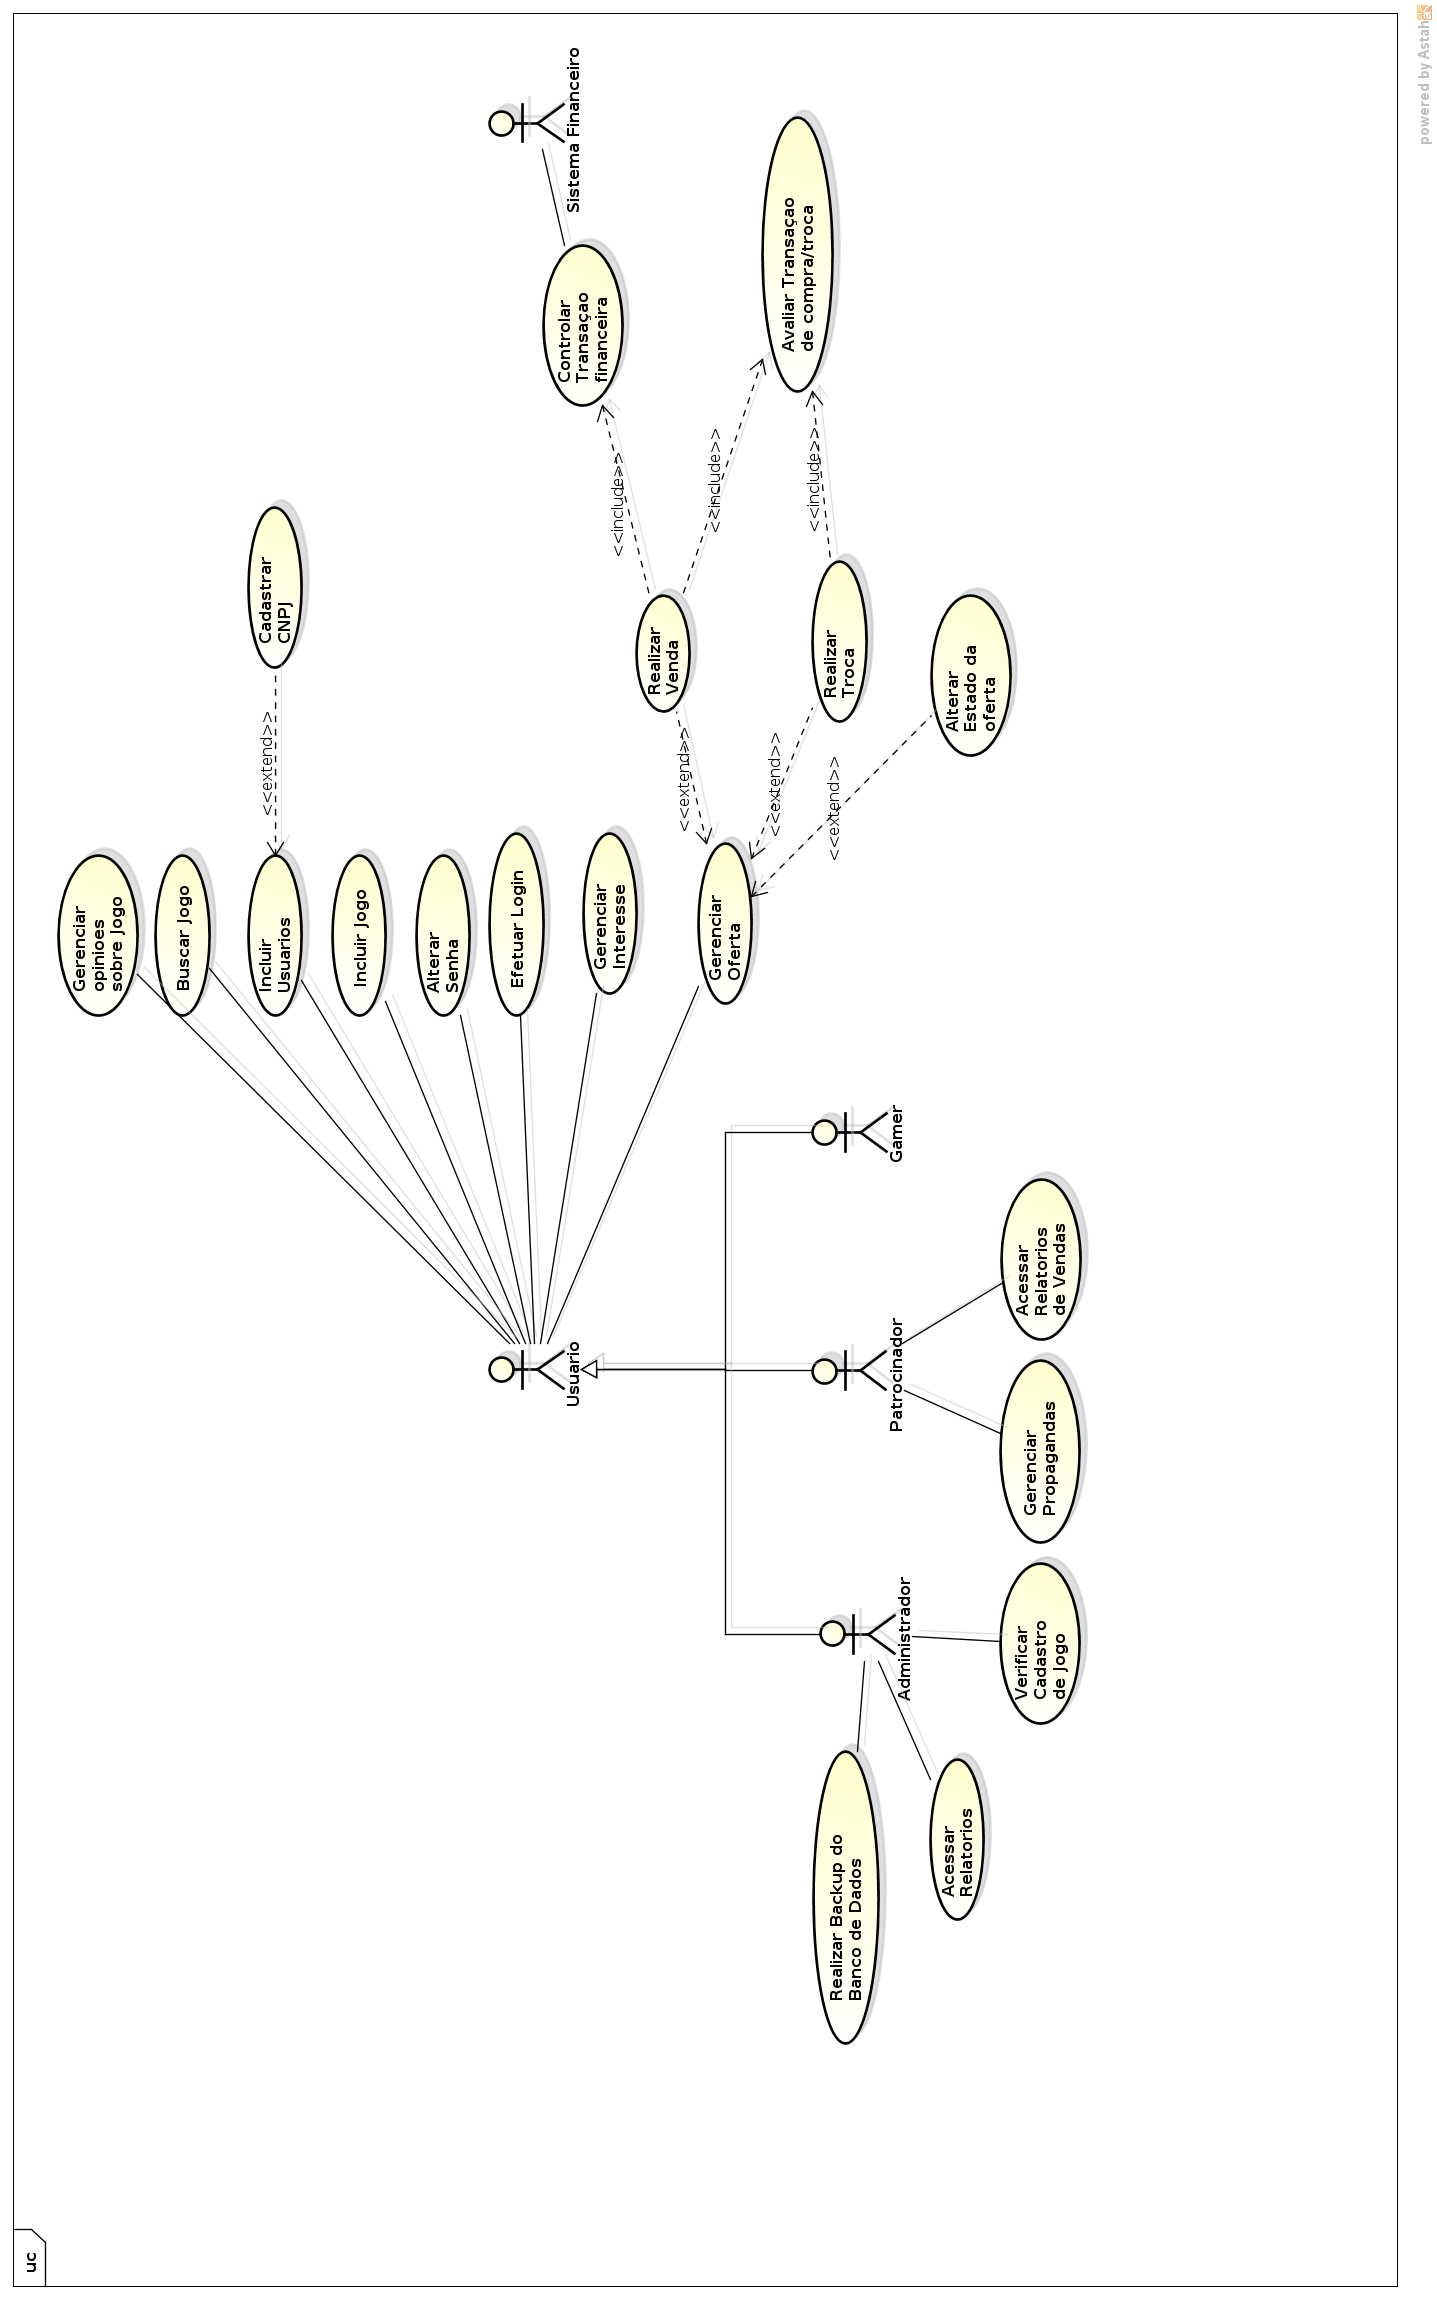
\includegraphics[width=\textwidth,height=\dimexpr\textheight-3\baselineskip\relax,keepaspectratio]{Diagrama.png}
        	\caption{Diagrama de Casos de Uso}
     		\label{diagrama}
    	\end{figure}
    	

\end{document}
